  \let\negmedspace\undefined
\let\negthickspace\undefined
\documentclass[journal]{IEEEtran}
\usepackage[a5paper, margin=10mm, onecolumn]{geometry}
\usepackage{lmodern} 
\usepackage{tfrupee} 

\setlength{\headheight}{1cm} % Set the height of the header box
\setlength{\headsep}{0mm}     % Set the distance between the header box and the top of the text

\usepackage{gvv-book}
\usepackage{gvv}
\usepackage{cite}
\usepackage{amsmath,amssymb,amsfonts,amsthm}
\usepackage{algorithmic}
\usepackage{graphicx}
\usepackage{textcomp}
\usepackage{xcolor}
\usepackage{txfonts}
\usepackage{listings}
\usepackage{enumitem}
\usepackage{mathtools}
\usepackage{gensymb}
\usepackage{comment}
\usepackage[breaklinks=true]{hyperref}
\usepackage{tkz-euclide} 
\usepackage{listings}                                      
\def\inputGnumericTable{}                                 
\usepackage[latin1]{inputenc}                                
\usepackage{color}                                            
\usepackage{array}                                            
\usepackage{longtable}
\usepackage{multicol}
\usepackage{calc}                                             
\usepackage{multirow}                                         
\usepackage{hhline}                                           
\usepackage{ifthen}                                           
\usepackage{lscape}
\begin{document}

\bibliographystyle{IEEEtran}
\vspace{3cm}

\title{4.3.20}
\author {EE25BTECH11031 - Sai Sreevallabh}
% \maketitle
% \newpage
% \bigskip
{\let\newpage\relax\maketitle}

\renewcommand{\thefigure}{\theenumi}
\renewcommand{\thetable}{\theenumi}
\setlength{\intextsep}{10pt} % Space between text and floats


\numberwithin{equation}{enumi}
\numberwithin{figure}{enumi}
\renewcommand{\thetable}{\theenumi}

\textbf{Question: }\\

Find the ratio in which the Y-axis divides the line segment joining the points $\brak{5,-6}$ and $\brak{-1,-4}$. Also find the point of intersection. \\

\textbf{Solution: }\\

Given points are\\
\begin{align}
    \vec{A}=\myvec{5\\-6} \ \text{and}\  \vec{B}=\myvec{-1\\-4}
\end{align}

Let $\vec{P}$ be a point on the Y-axis. We can assume it to be

\begin{align}
    \vec{P}=\myvec{0\\y}
\end{align}

$\vec{A}$, $\vec{B}$ and $\vec{P}$ are collinear. 

\begin{align}
    \vec{P}-\vec{A}=\myvec{-5 \\ y+6} \ , \ 
    \vec{B}-\vec{A}=\myvec{-6\\2}  
\end{align}

\begin{align}
    \myvec{\vec{P}-\vec{A} & \vec{B}-\vec{A}}^T =& \myvec{-5 & -6\\ y+6 & 2}^T\\
    =& \myvec{-5 & y+6 \\ -6 & 2}
\end{align}

Converting into echelon form using row operations

\begin{align}
    \myvec{x-1 & -3 \\ 3 & 2}\ \xleftrightarrow[]{R_2 \to R_2-\frac{6}{5}R_1} \  \myvec{-5 & y+6 \\ 0 & \frac{-6y-26}{5}}
\end{align}

The points are collinear. Hence the rank of the above matrix must be 1. So, 

\begin{align}
    &\frac{6y+26}{5} = 0\\
    \implies& y=-\frac{13}{3}
\end{align}\\

Let $\vec{P}$ divide the line joining points $\vec{A}$ and $\vec{B}$ in the ratio $k:1$. 

\begin{align}
    \vec{P}=\frac{k\vec{B}+\vec{A}}{k+1}
\end{align}

\begin{align}
    k\brak{\vec{P}- \vec{B}} = \vec{A}-\vec{P}
\end{align}

\begin{align}
    k=\frac{\brak{\vec{P}-\vec{B}}^T\brak{\vec{A}-\vec{P}}}{||\brak{\vec{P}-\vec{B}}||^2}
\end{align}

\begin{align}
      k=\frac{\myvec{1 & y+4}\myvec{5\\-y-6}}{{\norm{\myvec{1 \\ y+4}}}^2}
\end{align}

Substituting the value of $y$ as $-\frac{13}{3}$, we get the value of k as

\begin{align}
    k=5
\end{align}

$\therefore$ The point $\vec{P}\myvec{0\\-\frac{13}{3}}$ on the X-axis divides the line segment in the ratio $5:1$. 

\begin{figure}[h]
    \centering
    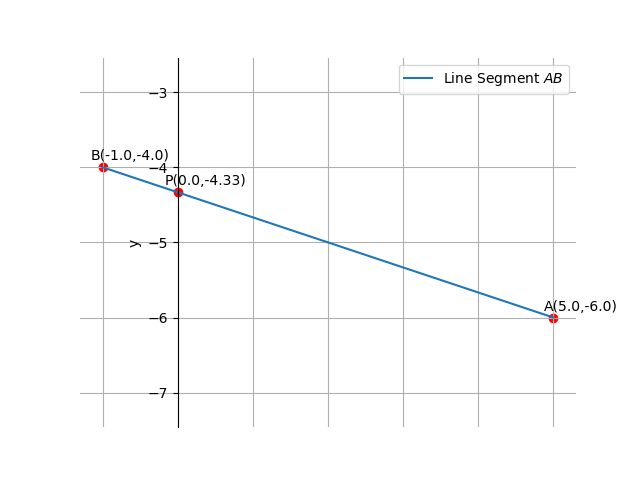
\includegraphics[width=1\columnwidth]{Figs/plot(py).png}
\end{figure}

\end{document}
